\section{Ejercicio 5}
  		Computaciones para el programa
  		\begin{verbatim}
		J(2,3,5)
		S(1)
		S(3)
		J(1,1,1)
  		\end{verbatim}
  		\subsection{Computación para la entrada $R1=0$, $R2=0$}
  		\begin{equation*}\begin{gathered}
		(1, <R1=0, R2=0, R3=0>) \sim (5, <R1=0, R2=0, R3=0>)
		\end{gathered}\end{equation*}
		\begin{figure}[H]
  			\centering
  			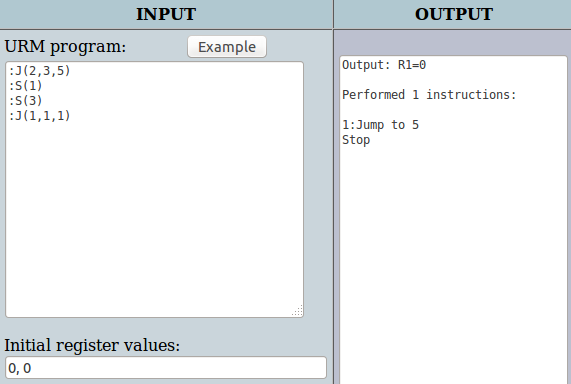
\includegraphics[scale=0.5]{images/500.png}
  		\end{figure}
		\subsection{Computación para la entrada $R1=1$, $R2=0$}
		\begin{equation*}\begin{gathered}
		(1, <R1=1, R2=0, R3=0>) \sim (5, <R1=1, R2=0, R3=0>)
		\end{gathered}\end{equation*}
		\begin{figure}[H]
  			\centering
  			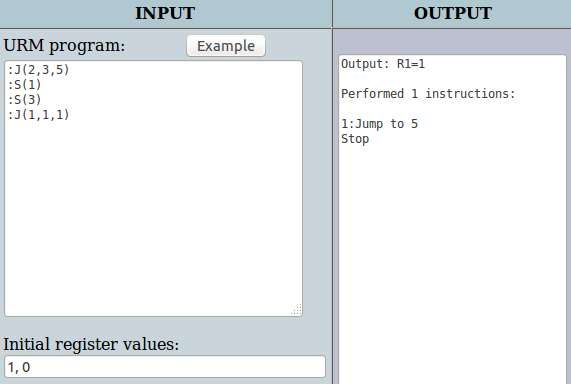
\includegraphics[scale=0.5]{images/510.png}
  		\end{figure}
		\subsection{Computación para la entrada $R1=0$, $R2=1$}
		\begin{equation*}\begin{gathered}
		(1, <R1=0, R2=1, R3=0>) \sim (2, <R1=0, R2=1, R3=0>) \sim (3, <R1=1, R2=1, R3=0>) \sim\\
		(4, <R1=1, R2=1, R3=1>) \sim (1, <R1=1, R2=1, R3=1>) \sim (5, <R1=1, R2=1, R3=1>)
		\end{gathered}\end{equation*}
		\begin{figure}[H]
  			\centering
  			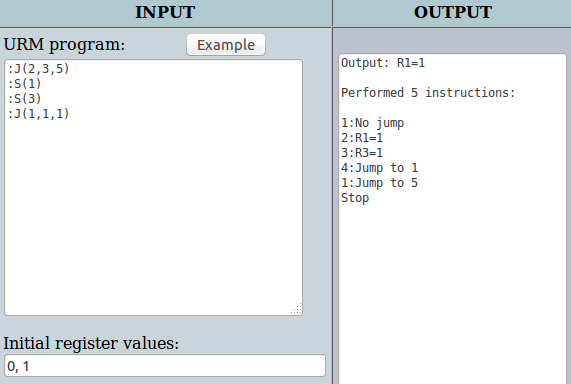
\includegraphics[scale=0.5]{images/501.png}
  		\end{figure}
		\subsection{Computación para la entrada $R1=1$, $R2=1$}
		\begin{equation*}\begin{gathered}
		(1, <R1=1, R2=1, R3=0>) \sim (2, <R1=1, R2=1, R3=0>) \sim (3, <R1=2, R2=1, R3=0>) \sim\\
		(4, <R1=2, R2=1, R3=1>) \sim (1, <R1=2, R2=1, R3=1>) \sim (5, <R1=2, R2=1, R3=1>)
		\end{gathered}\end{equation*}
		\begin{figure}[H]
  			\centering
  			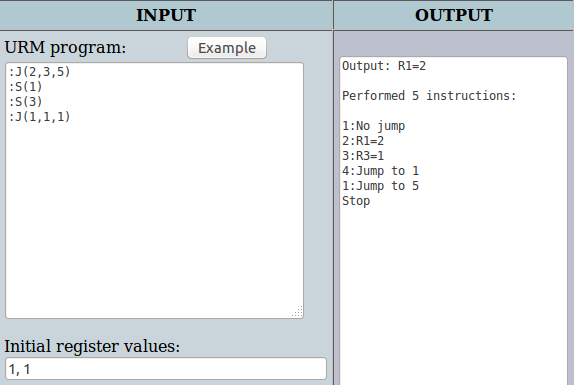
\includegraphics[scale=0.5]{images/511.png}
  		\end{figure}
		\subsection{Función calculada}
		El programa calcula la función
		\begin{equation*}
  			f(x_1, x_2) = x_1+x_2
  		\end{equation*}
